\chapter{Formulierung von Problemen und L�sungen in der Symbolischen Informationsverarbeitung}

Um Probleme mit Hilfe von KI zu l�sen, m�ssen sie zun�chst in einer Weise dargestellt werden, die von Computern verarbeitet werden kann. Dies kann mit herk�mmlichen Programmiersprachen �ber symbolische Informationsverarbeitung geschehen

\section{Tpyische KI-Problemstellungen}


Viele Probleme k�nnen mit Hilfe von KI gel�st werden. Die h?ufigsten sind:
\begin{itemize}
    \item \textbf{Navigation} z.B: Labyrinth/Navigationsspiele, autonomer Staubsauger, Wegplanung
    \item \textbf{Strategiespiele} z.B: Brettspiele, Puzzle
    \item \textbf{Komplexe Aufgaben} z.B: Robocup (Navigation + Strategie)
\end{itemize}

\section{Probleml�sung mit KI}

\subsection{Schritte um Probleme zu l�sen}

\begin{enumerate}
    \item Zielformulierung:
    \begin{itemize}
        \item Soweit m�glich, Plausibilit�ts-Check dabei durchf�hren: Ist das Ziel machbar?
        \item \textbf{Beispiel:} Hans will von A nach B, kennt aber den Weg nicht.
    \end{itemize}
    \item Problemformulierung
    \begin{itemize}
        \item Ausgangssituation formulieren.
        \item feststellen welche Operationen m�glich sind (z.B Spielregeln).
        \item \textbf{Beispiel:} Durch ausf�hren von Fahr-Aktionen von A �ber verbundene Nachbarorte nach B kommen. M�gliche Operationen w�ren: in die benachbarten St�dte zu fahren.
    \end{itemize}
    \item Konstruktion einer L�sung
    \begin{itemize}
        \item bewerte G�te einer L�sung
        \item w�hle effektiven L�sungsweg
        \item \textbf{Beispiel:} Ein m�glicher Weg zur L�sung des Problems w�re die Erstellung eines Suchbaums.
    \end{itemize}
    \item Ausf�hrung
    \begin{itemize}
        \item L�uft alles wie geplant?
    \end{itemize}
\end{enumerate}

\subsection{Performanzma� berechnen}

\begin{itemize}
    \item Oft gibt es mehrere zul�ssige L�sungswege zu einem Probleme
    \item Wie findet man die optimalste L�sung?
    \item Zur Bewertung der \textbf{G�te} einer L�sung berechnet man die Gesamtkosten
\end{itemize}

\[Gesamtkosten=Suchkosten + Pfadkosten\]

\begin{itemize}
    \item Es ist oft schwierig, die G�te einer L�sung zu verrechnen, da es oft viele m�gliche Aspekte gibt, die beobachtet und gemessen werden k�nnen.
    \item Manchmal ist es besser, die weniger optimale L�sung zu w�hlen, die schneller berechnet werden kann: Genauere Planung kann mehr Zeit kosten als sie erspart!
\end{itemize}

\section{Beispielformulierungen von Zielen und Problemen}

\subsection{8er Puzzle (Sliding block puzzle)}

\begin{itemize}
    \item Hochgradig kombinatorisches NP-vollst�ndiges Problem. Oft genutzt als Standardtest f�r neue Suchalgorithmen.
\end{itemize}

\begin{figure}[h!]
    \centering
    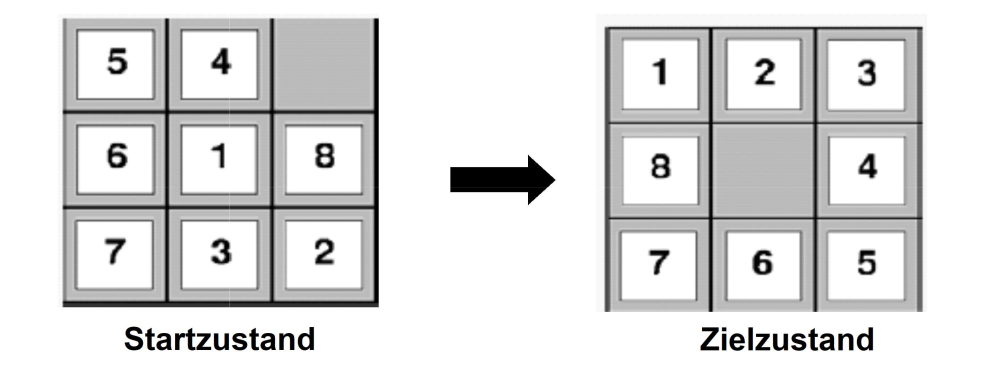
\includegraphics[width=0.8\textwidth]{figures/8er-puzzle.png}
    \caption{8er puzzle Start- und Zielzustand}
    \label{fig:8er-puzzle}
\end{figure}

\begin{itemize}
    \item Zust�nde: Lokalit�t der 8 Fliesen in eine der 9 Fl�chen plus eine freie Kachel
    \item Operatoren: Blank nach Links, Rechts, Auf, Ab 
    \item Ziel-test: Blank-Kachel in der Mitte
    \item Pfadkosten: jeder Schritt kostet eine Einheit
\end{itemize}

\subsection{Staubsauger-Roboter}

Vieles an der Implementierung dieses Roboters muss abstrahiert werden:
\begin{itemize}
    \item World States: Umfassen alle Aspekte der reelen Welt
    \item Problem States: Nur Aspekte der relevant f�r das Problem sind. Die Modellierung von diesen Aspekten erfolgt meist in Form \textbf{symbolisher} Beschreibungen. 
    \item Erstens m�ssen die m�glichen World States als Problem States dargestellt werden:
\end{itemize}

\begin{figure}[h!]
    \centering
    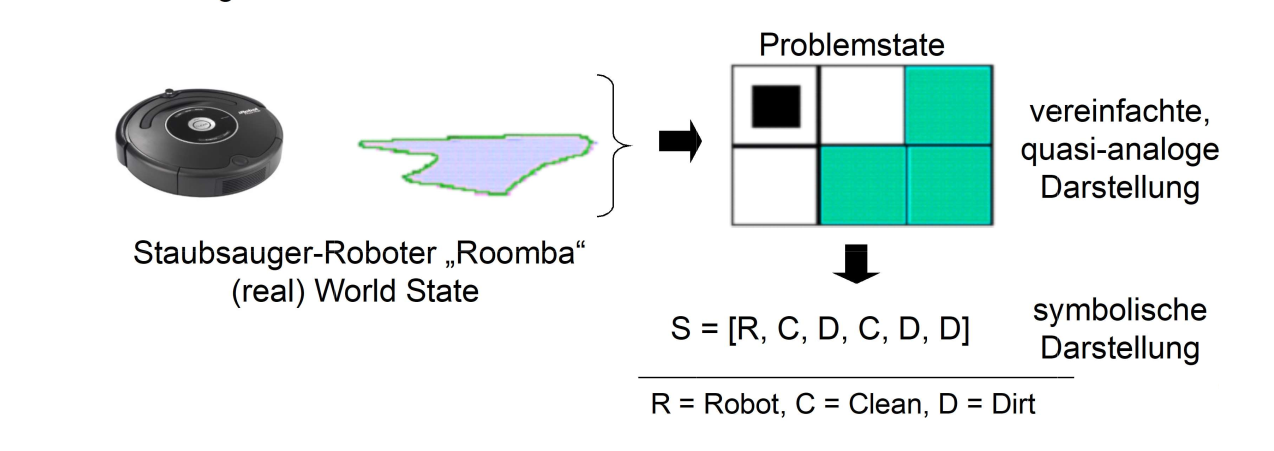
\includegraphics[width=0.8\textwidth]{figures/roomba-world-to-problem-states.png}
    \caption{Abbildung World States auf Problem States}
    \label{fig:roomba-abbildung}
\end{figure}
